\section{Regelungen}
\subsection{Glieder}
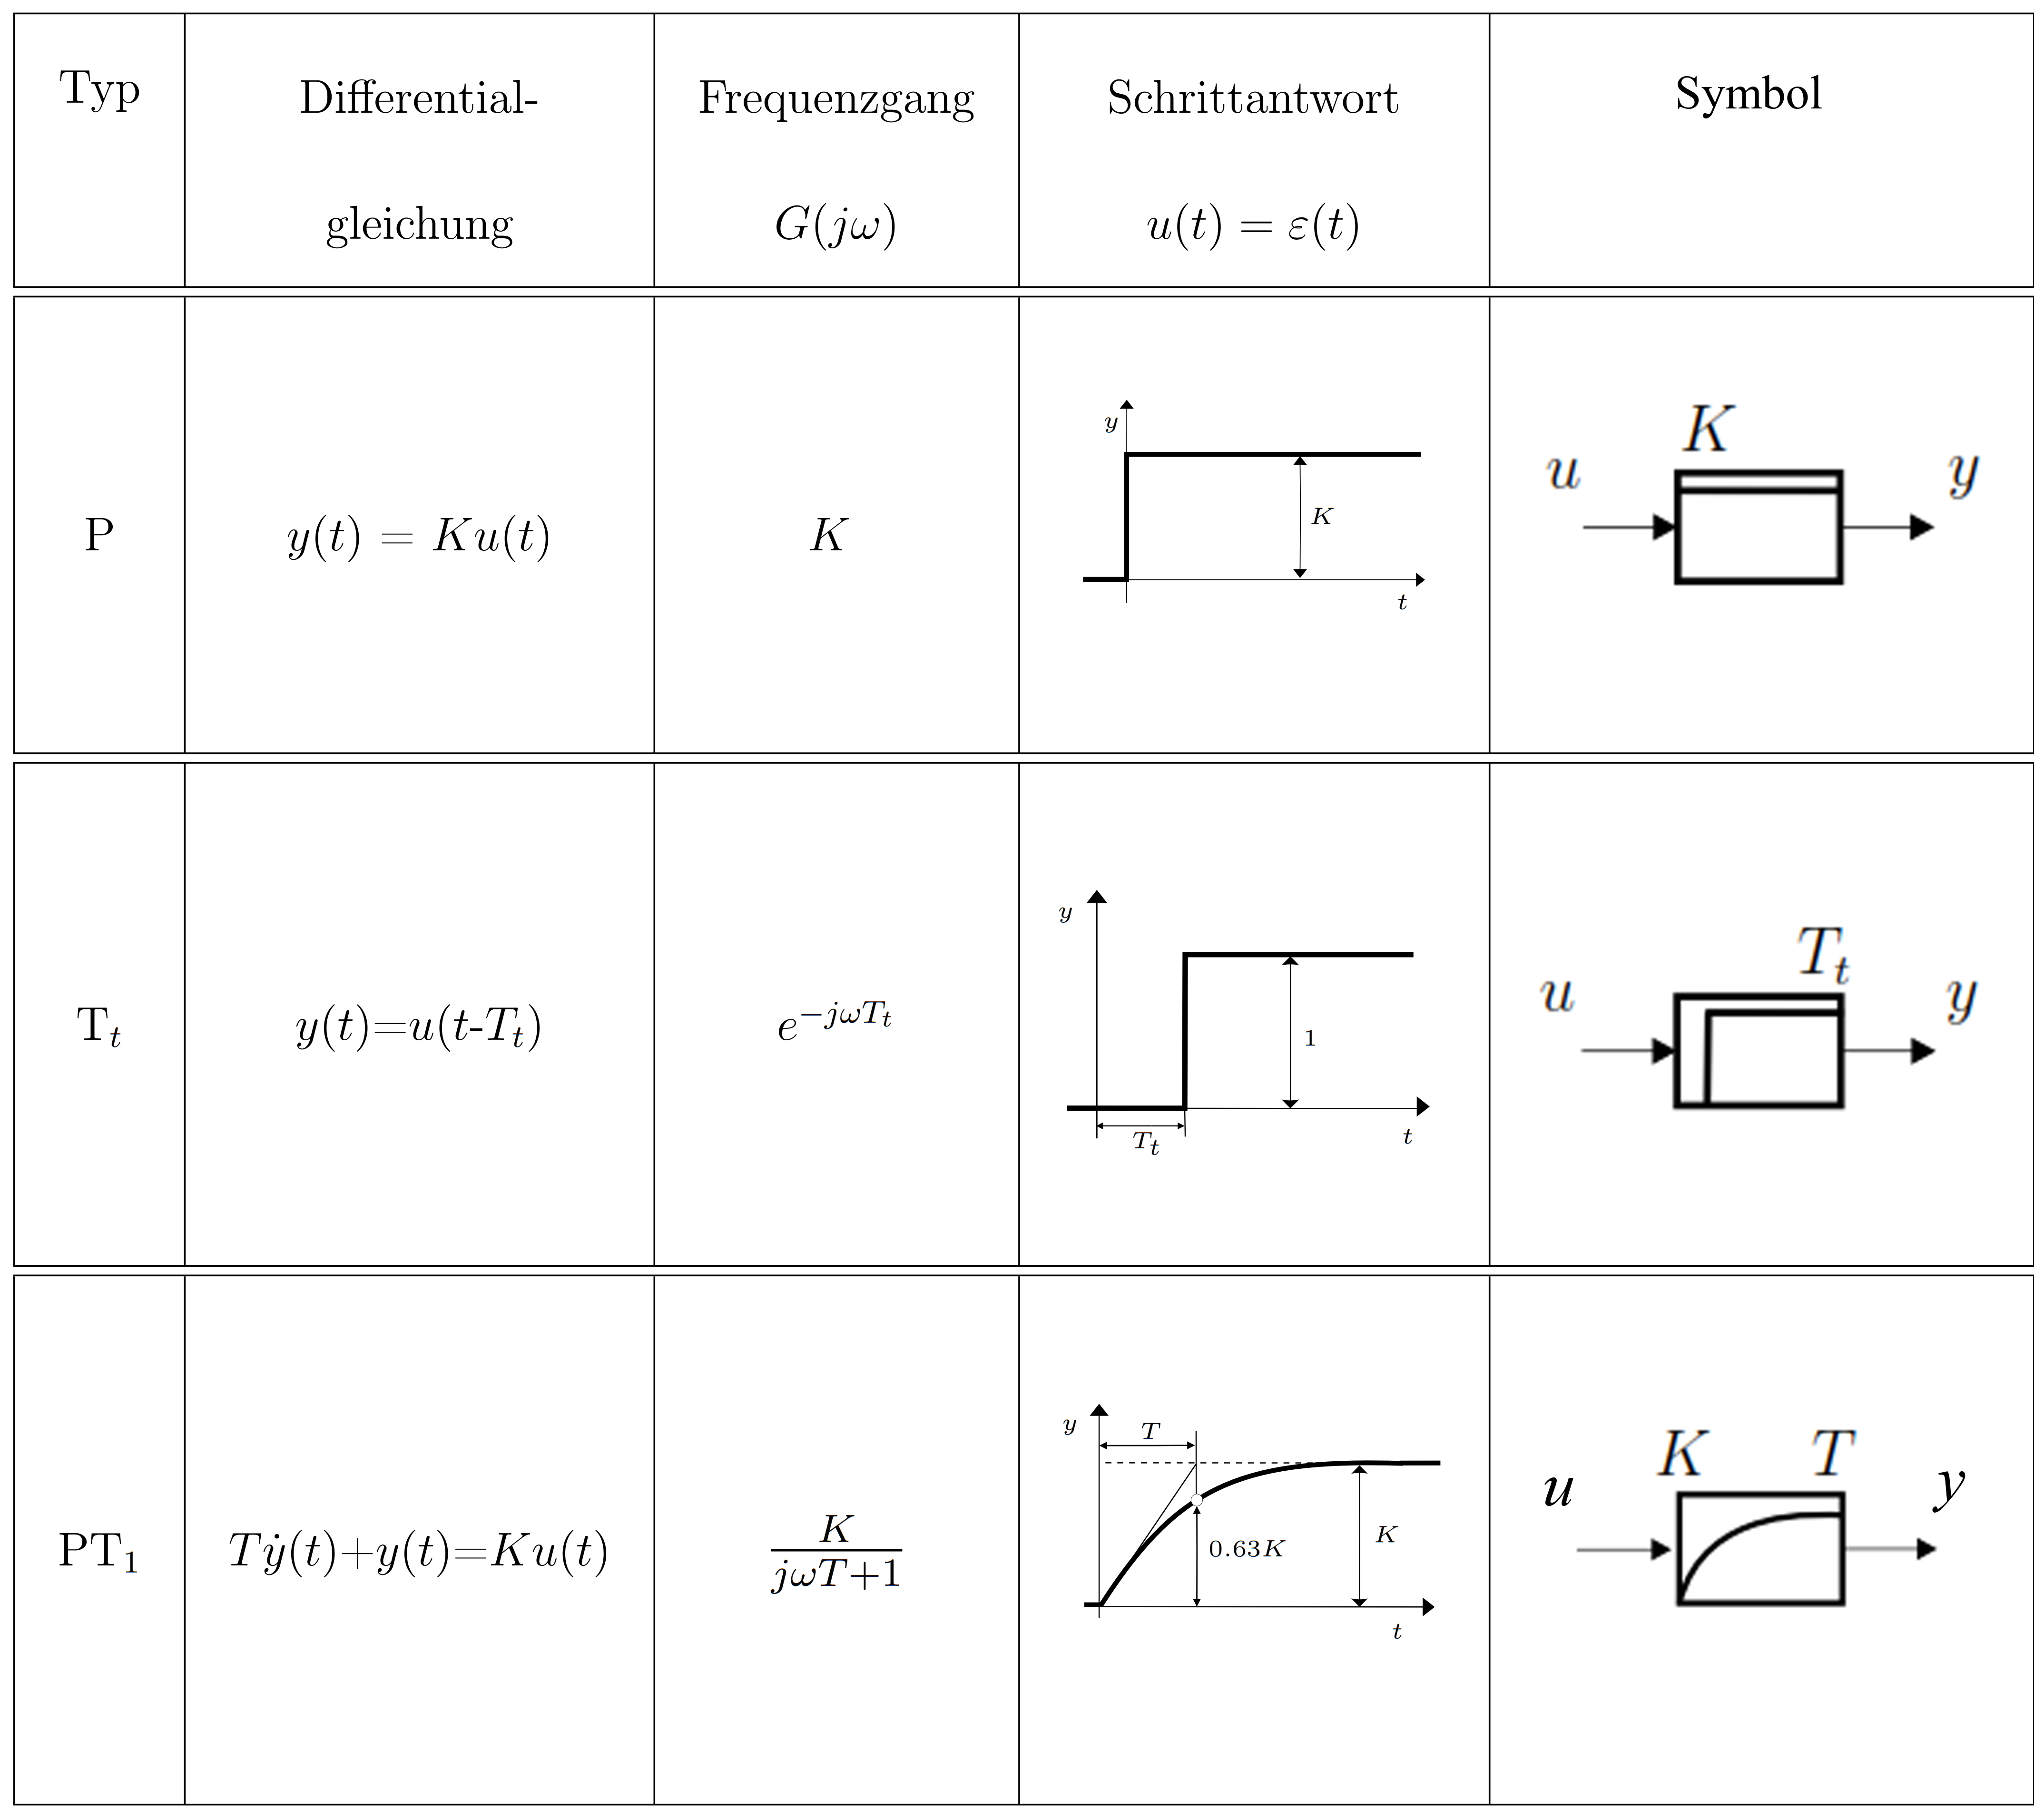
\includegraphics[width=12 cm]{./bilder/glieder1.png} \newpage
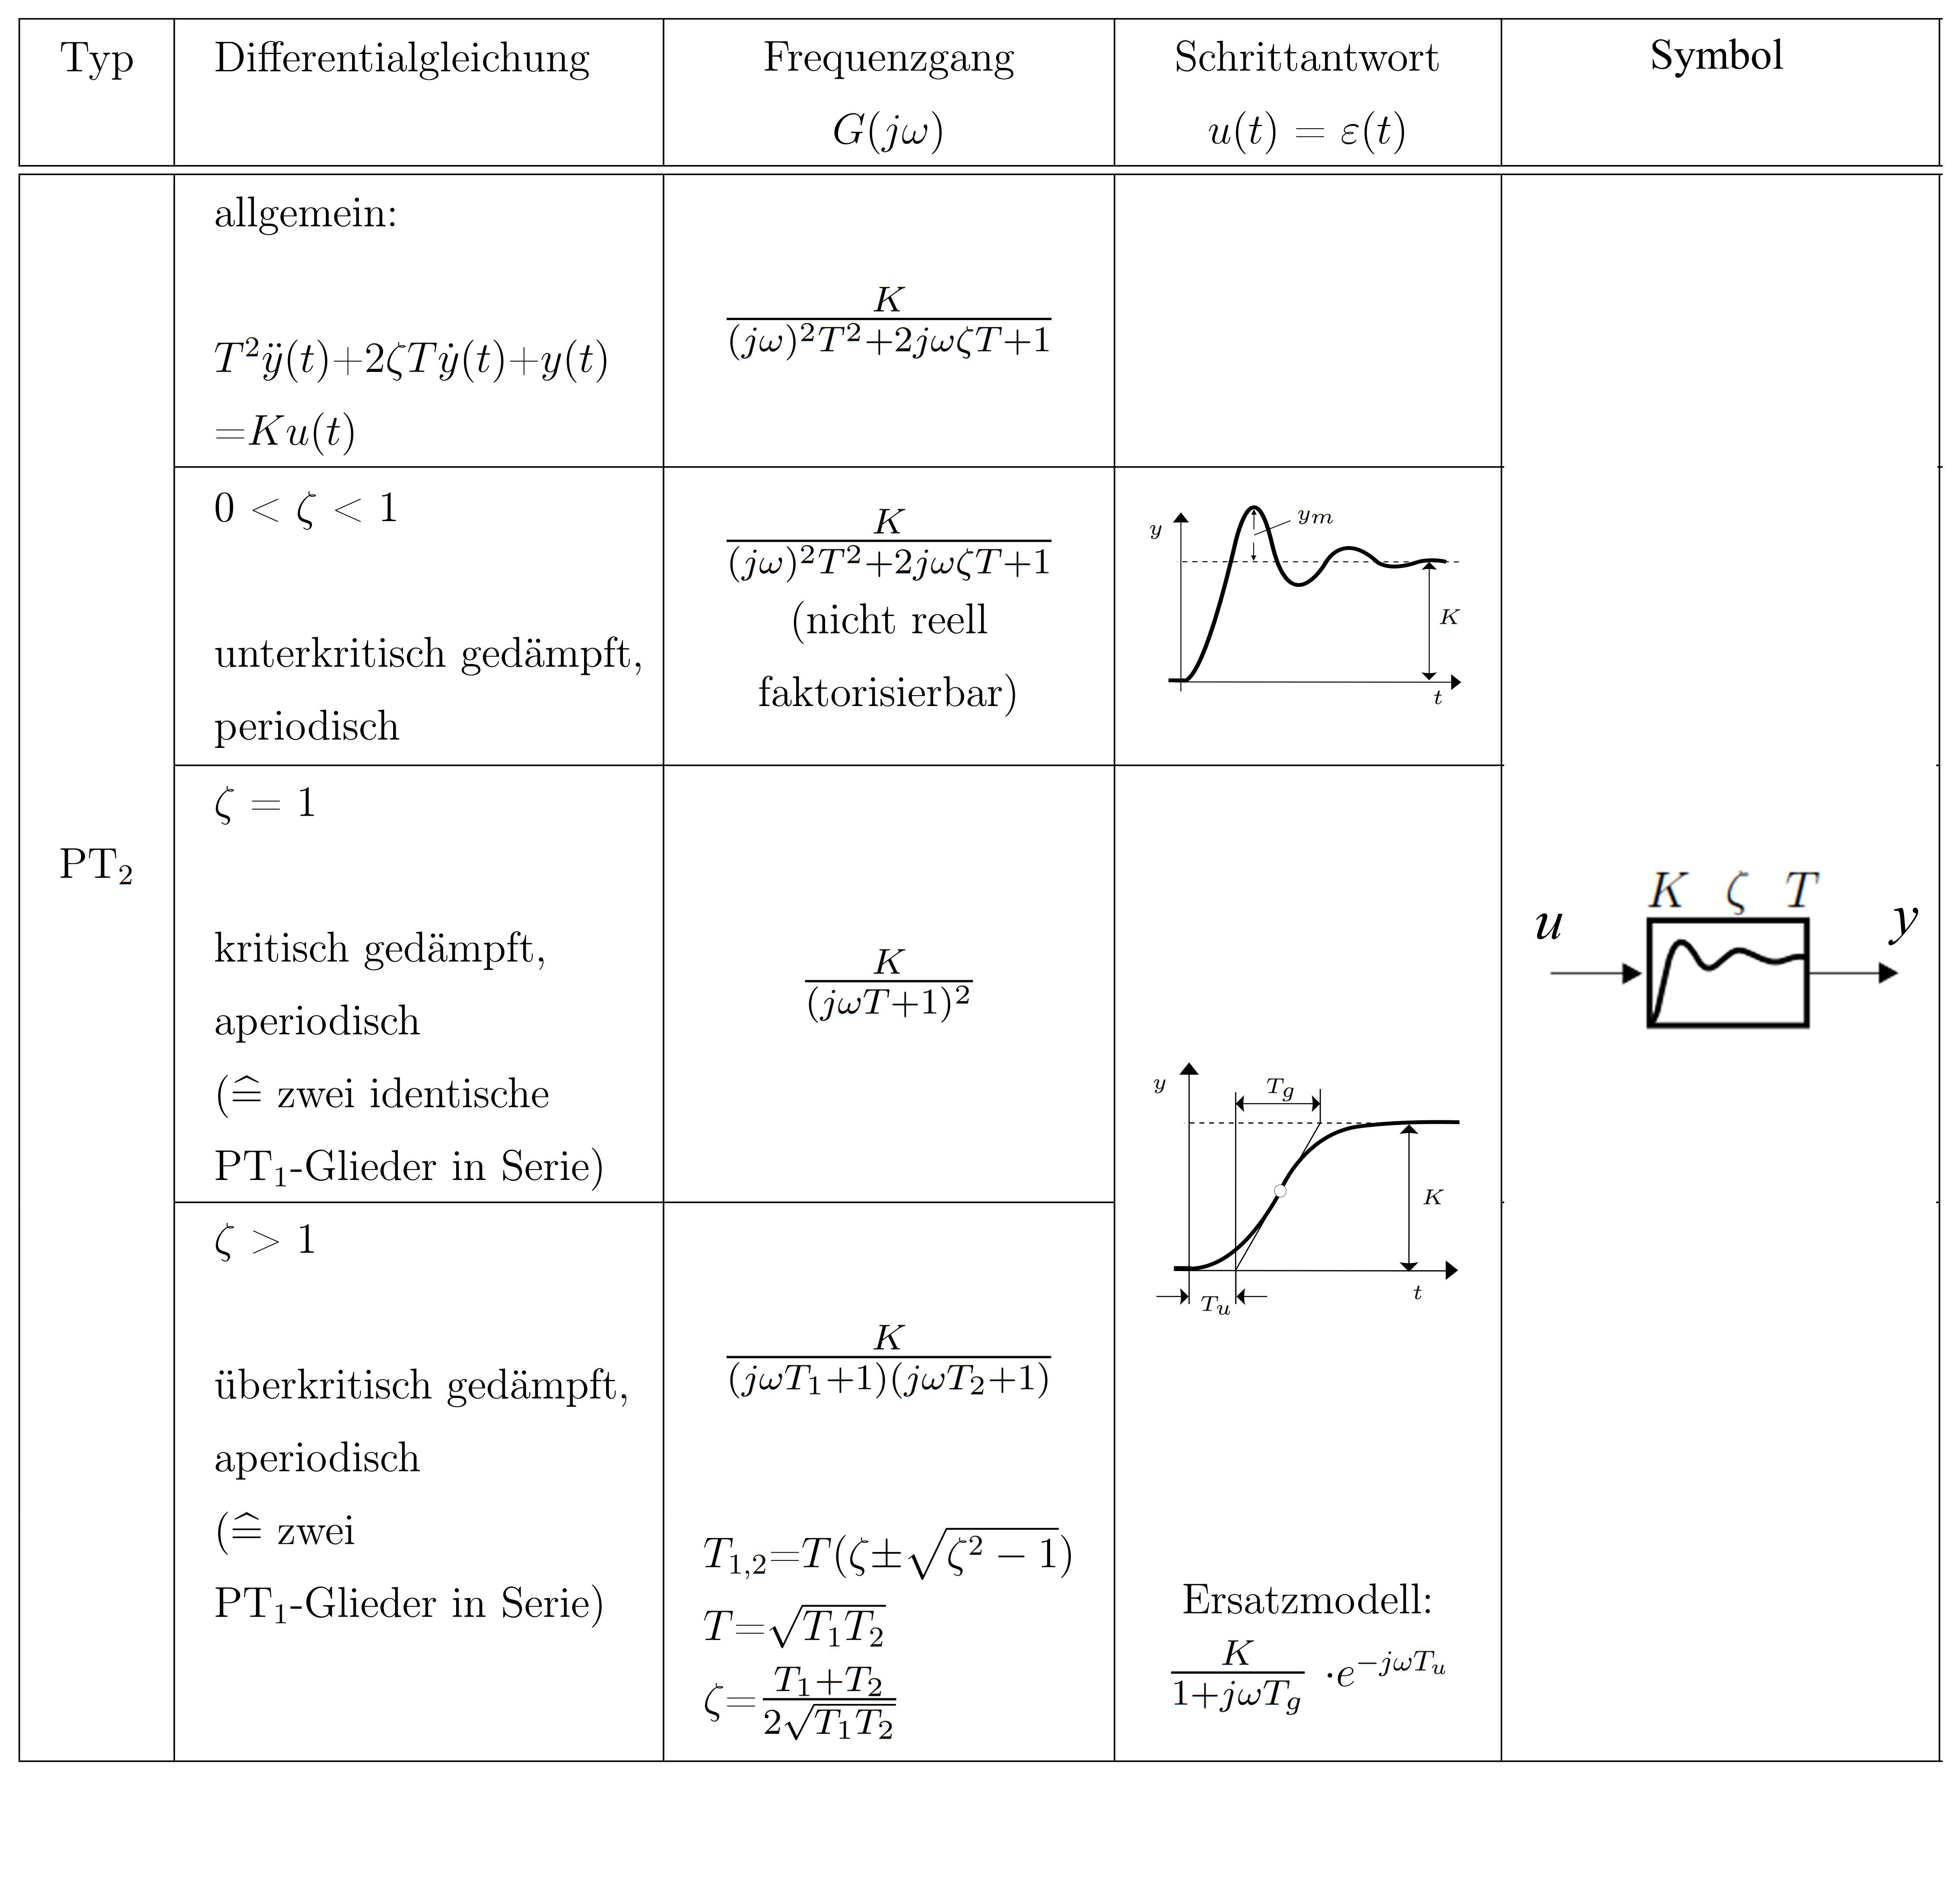
\includegraphics[width=12 cm]{./bilder/glieder2.png} \\\\
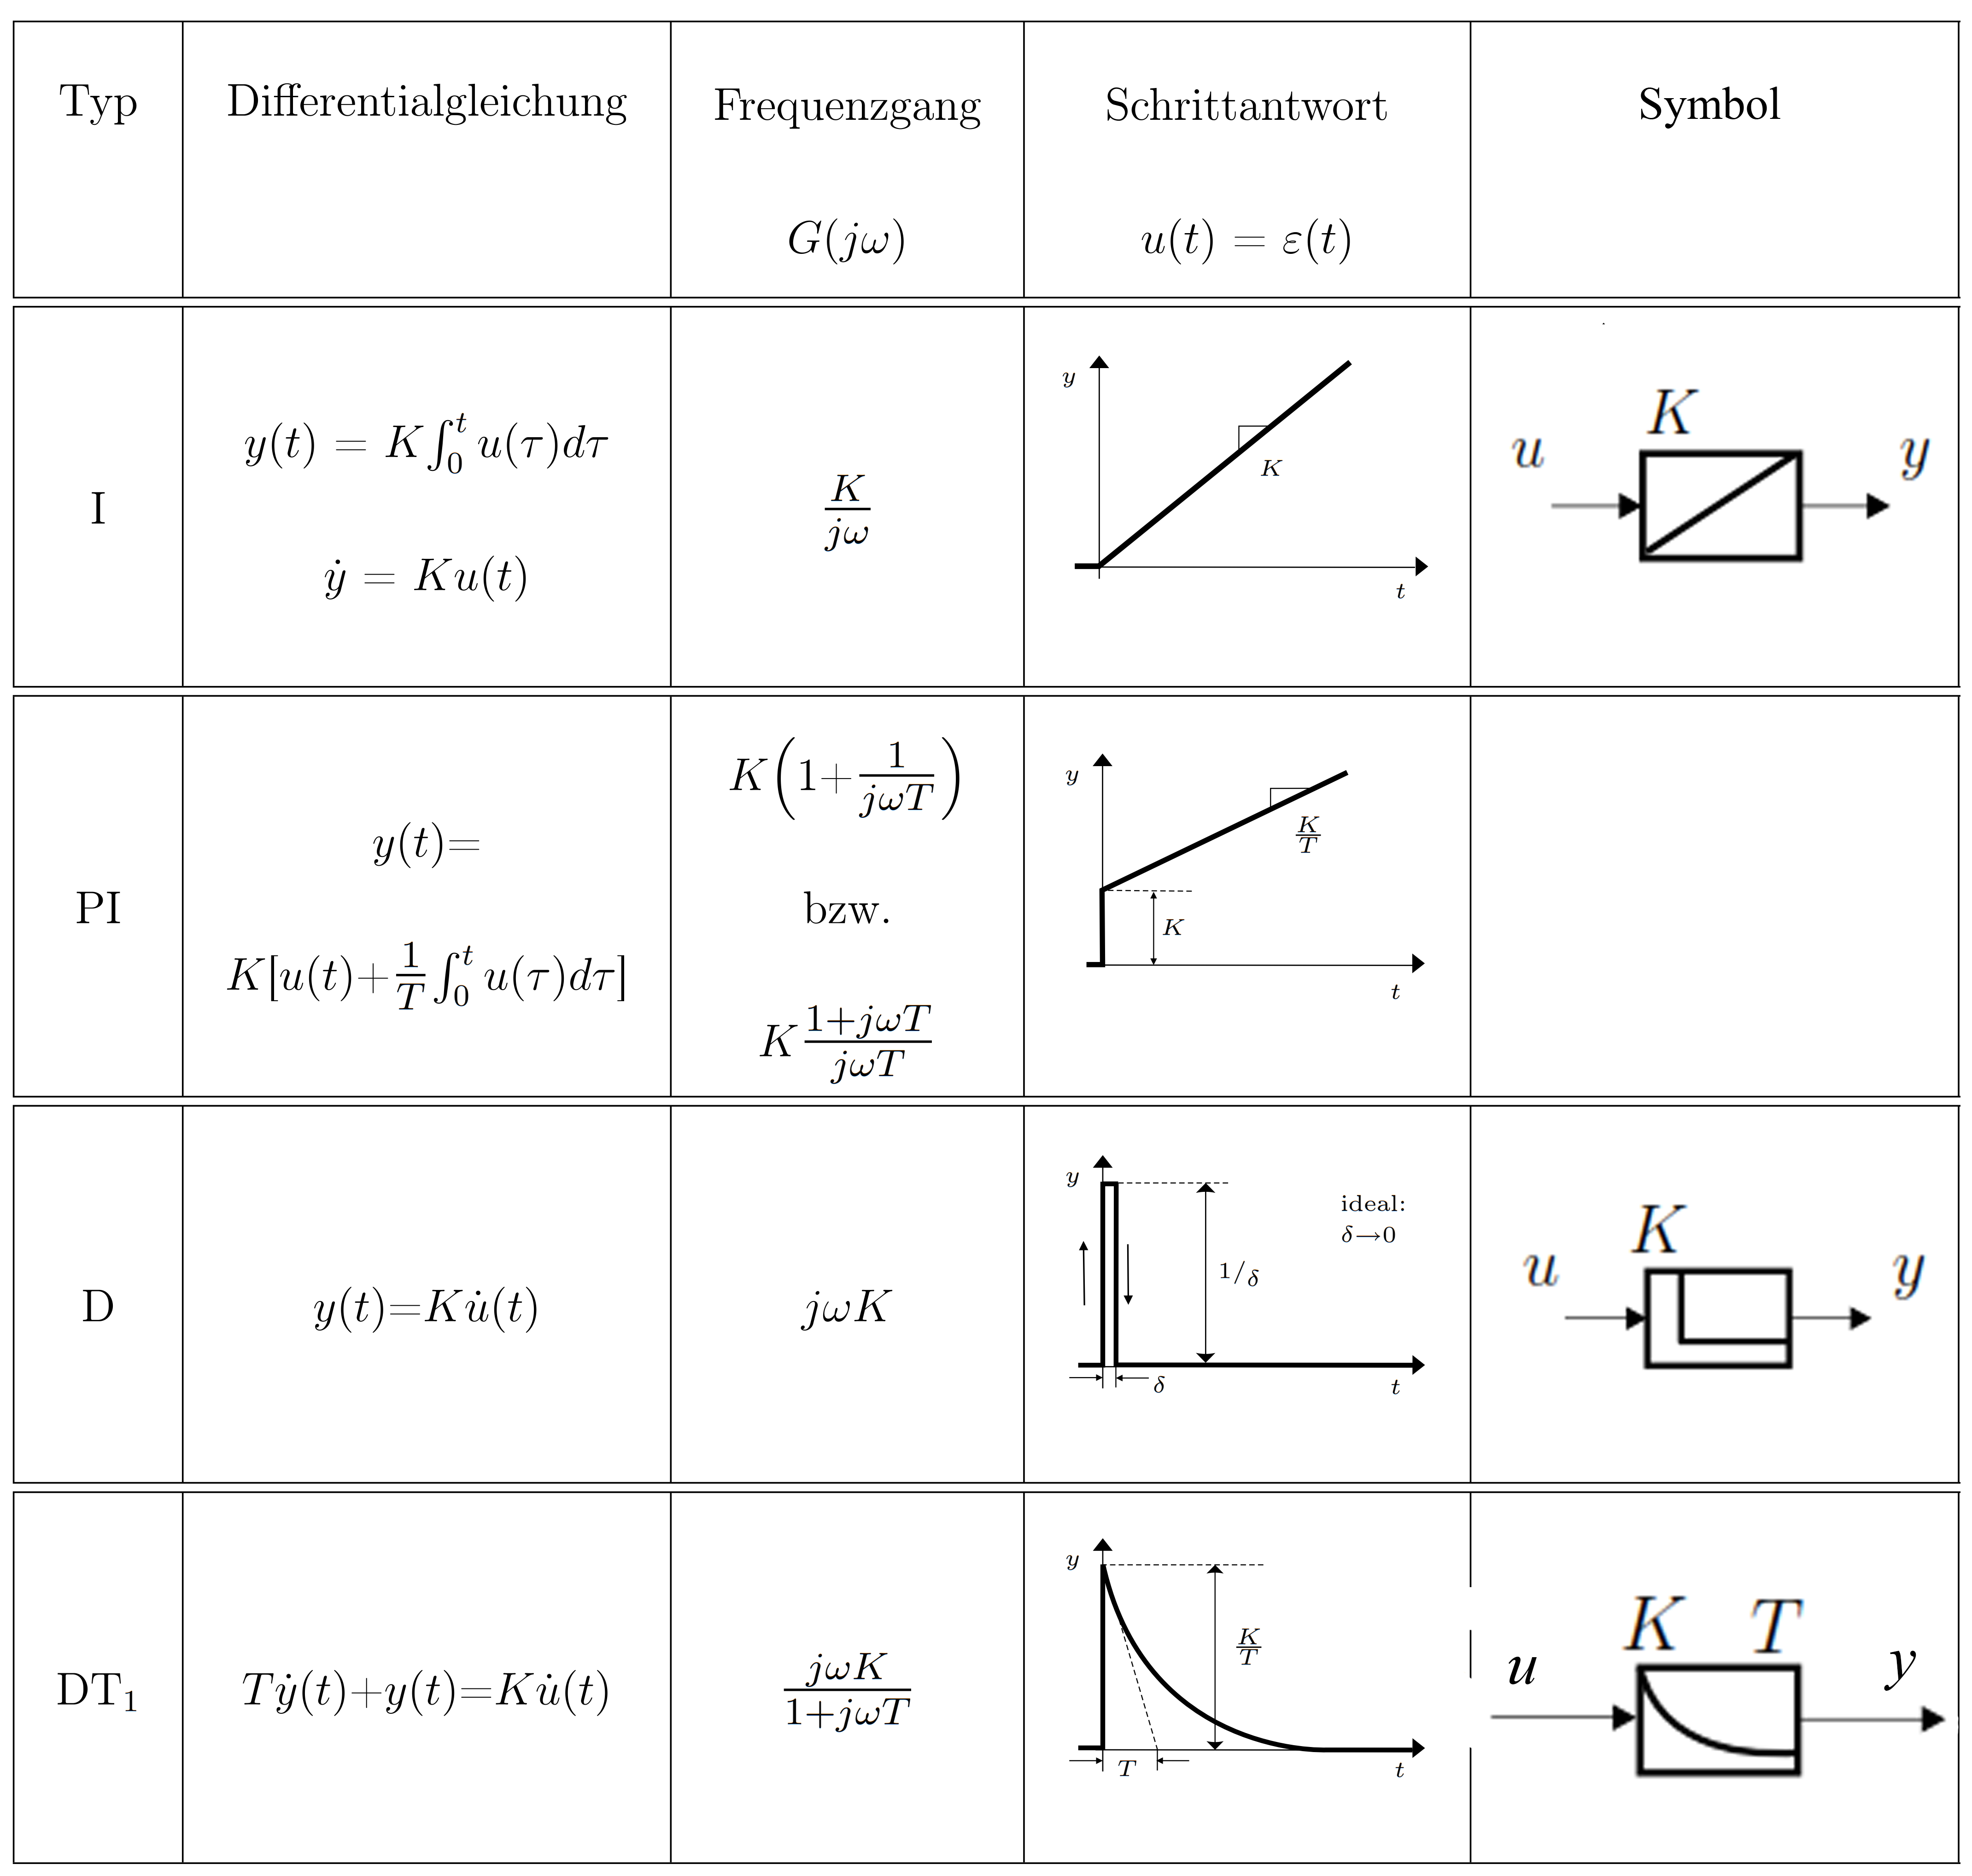
\includegraphics[width=12 cm]{./bilder/glieder3.png} \newpage
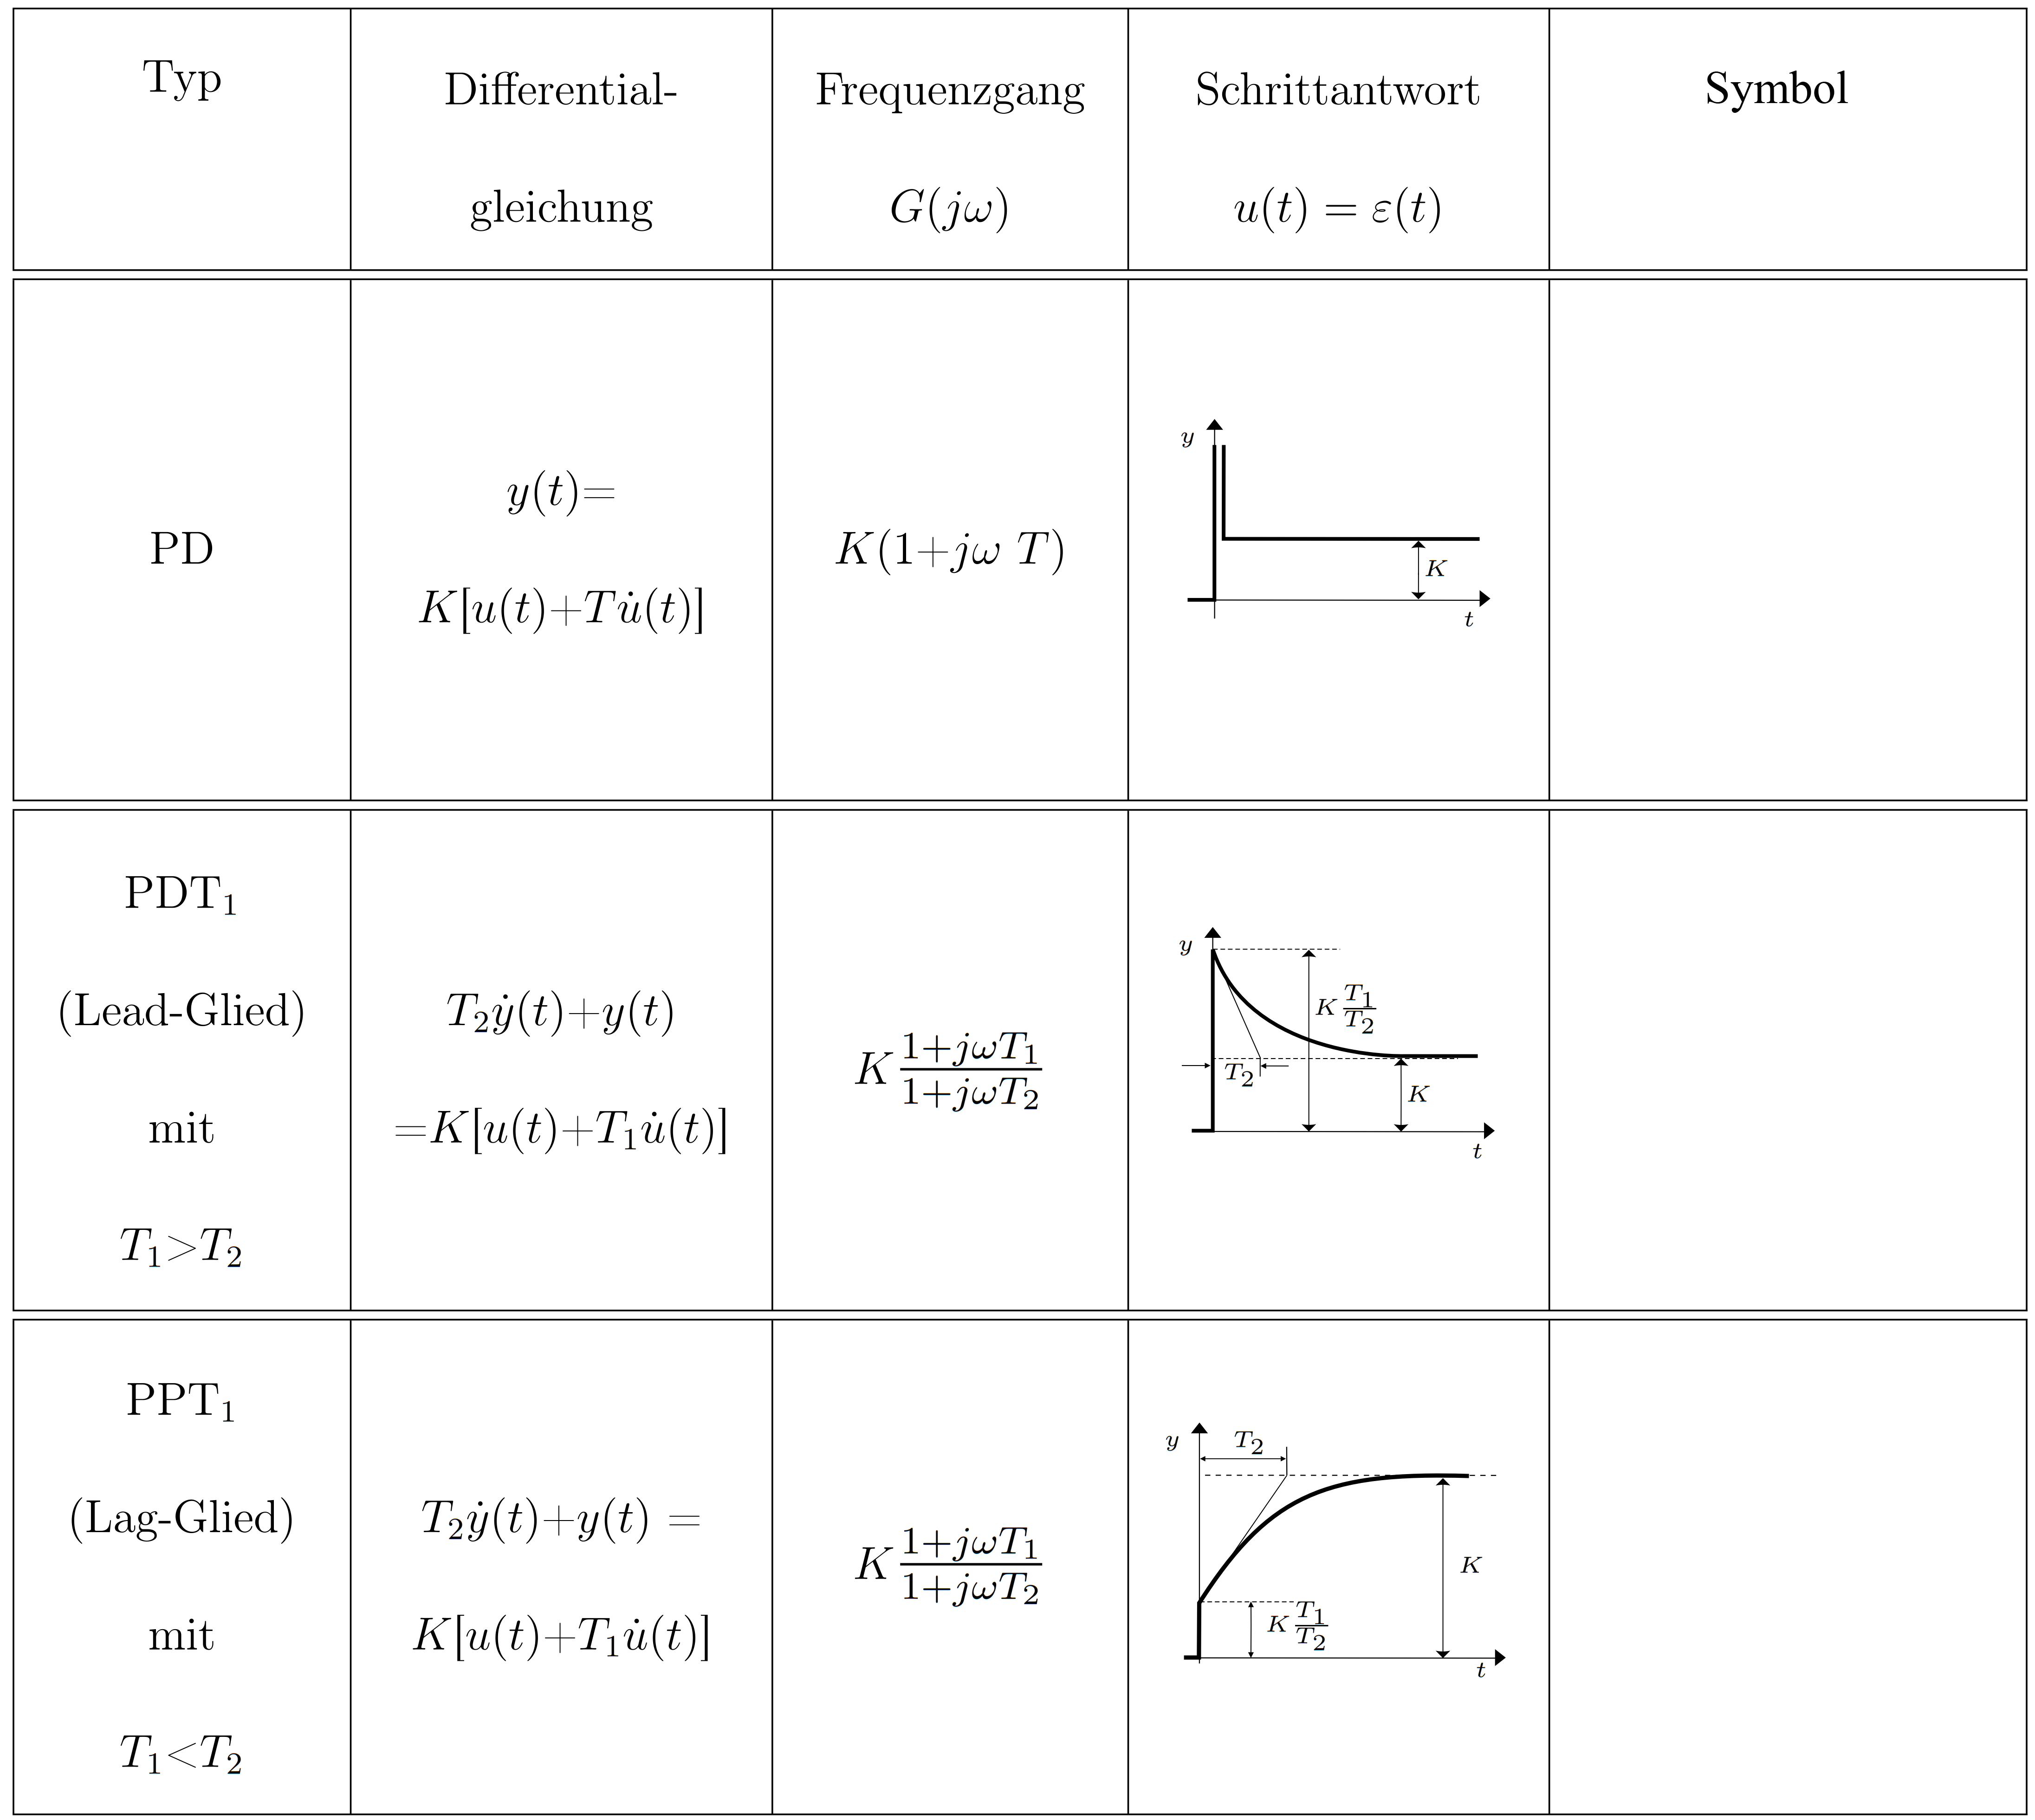
\includegraphics[width=12 cm]{./bilder/glieder4.png} \\\\
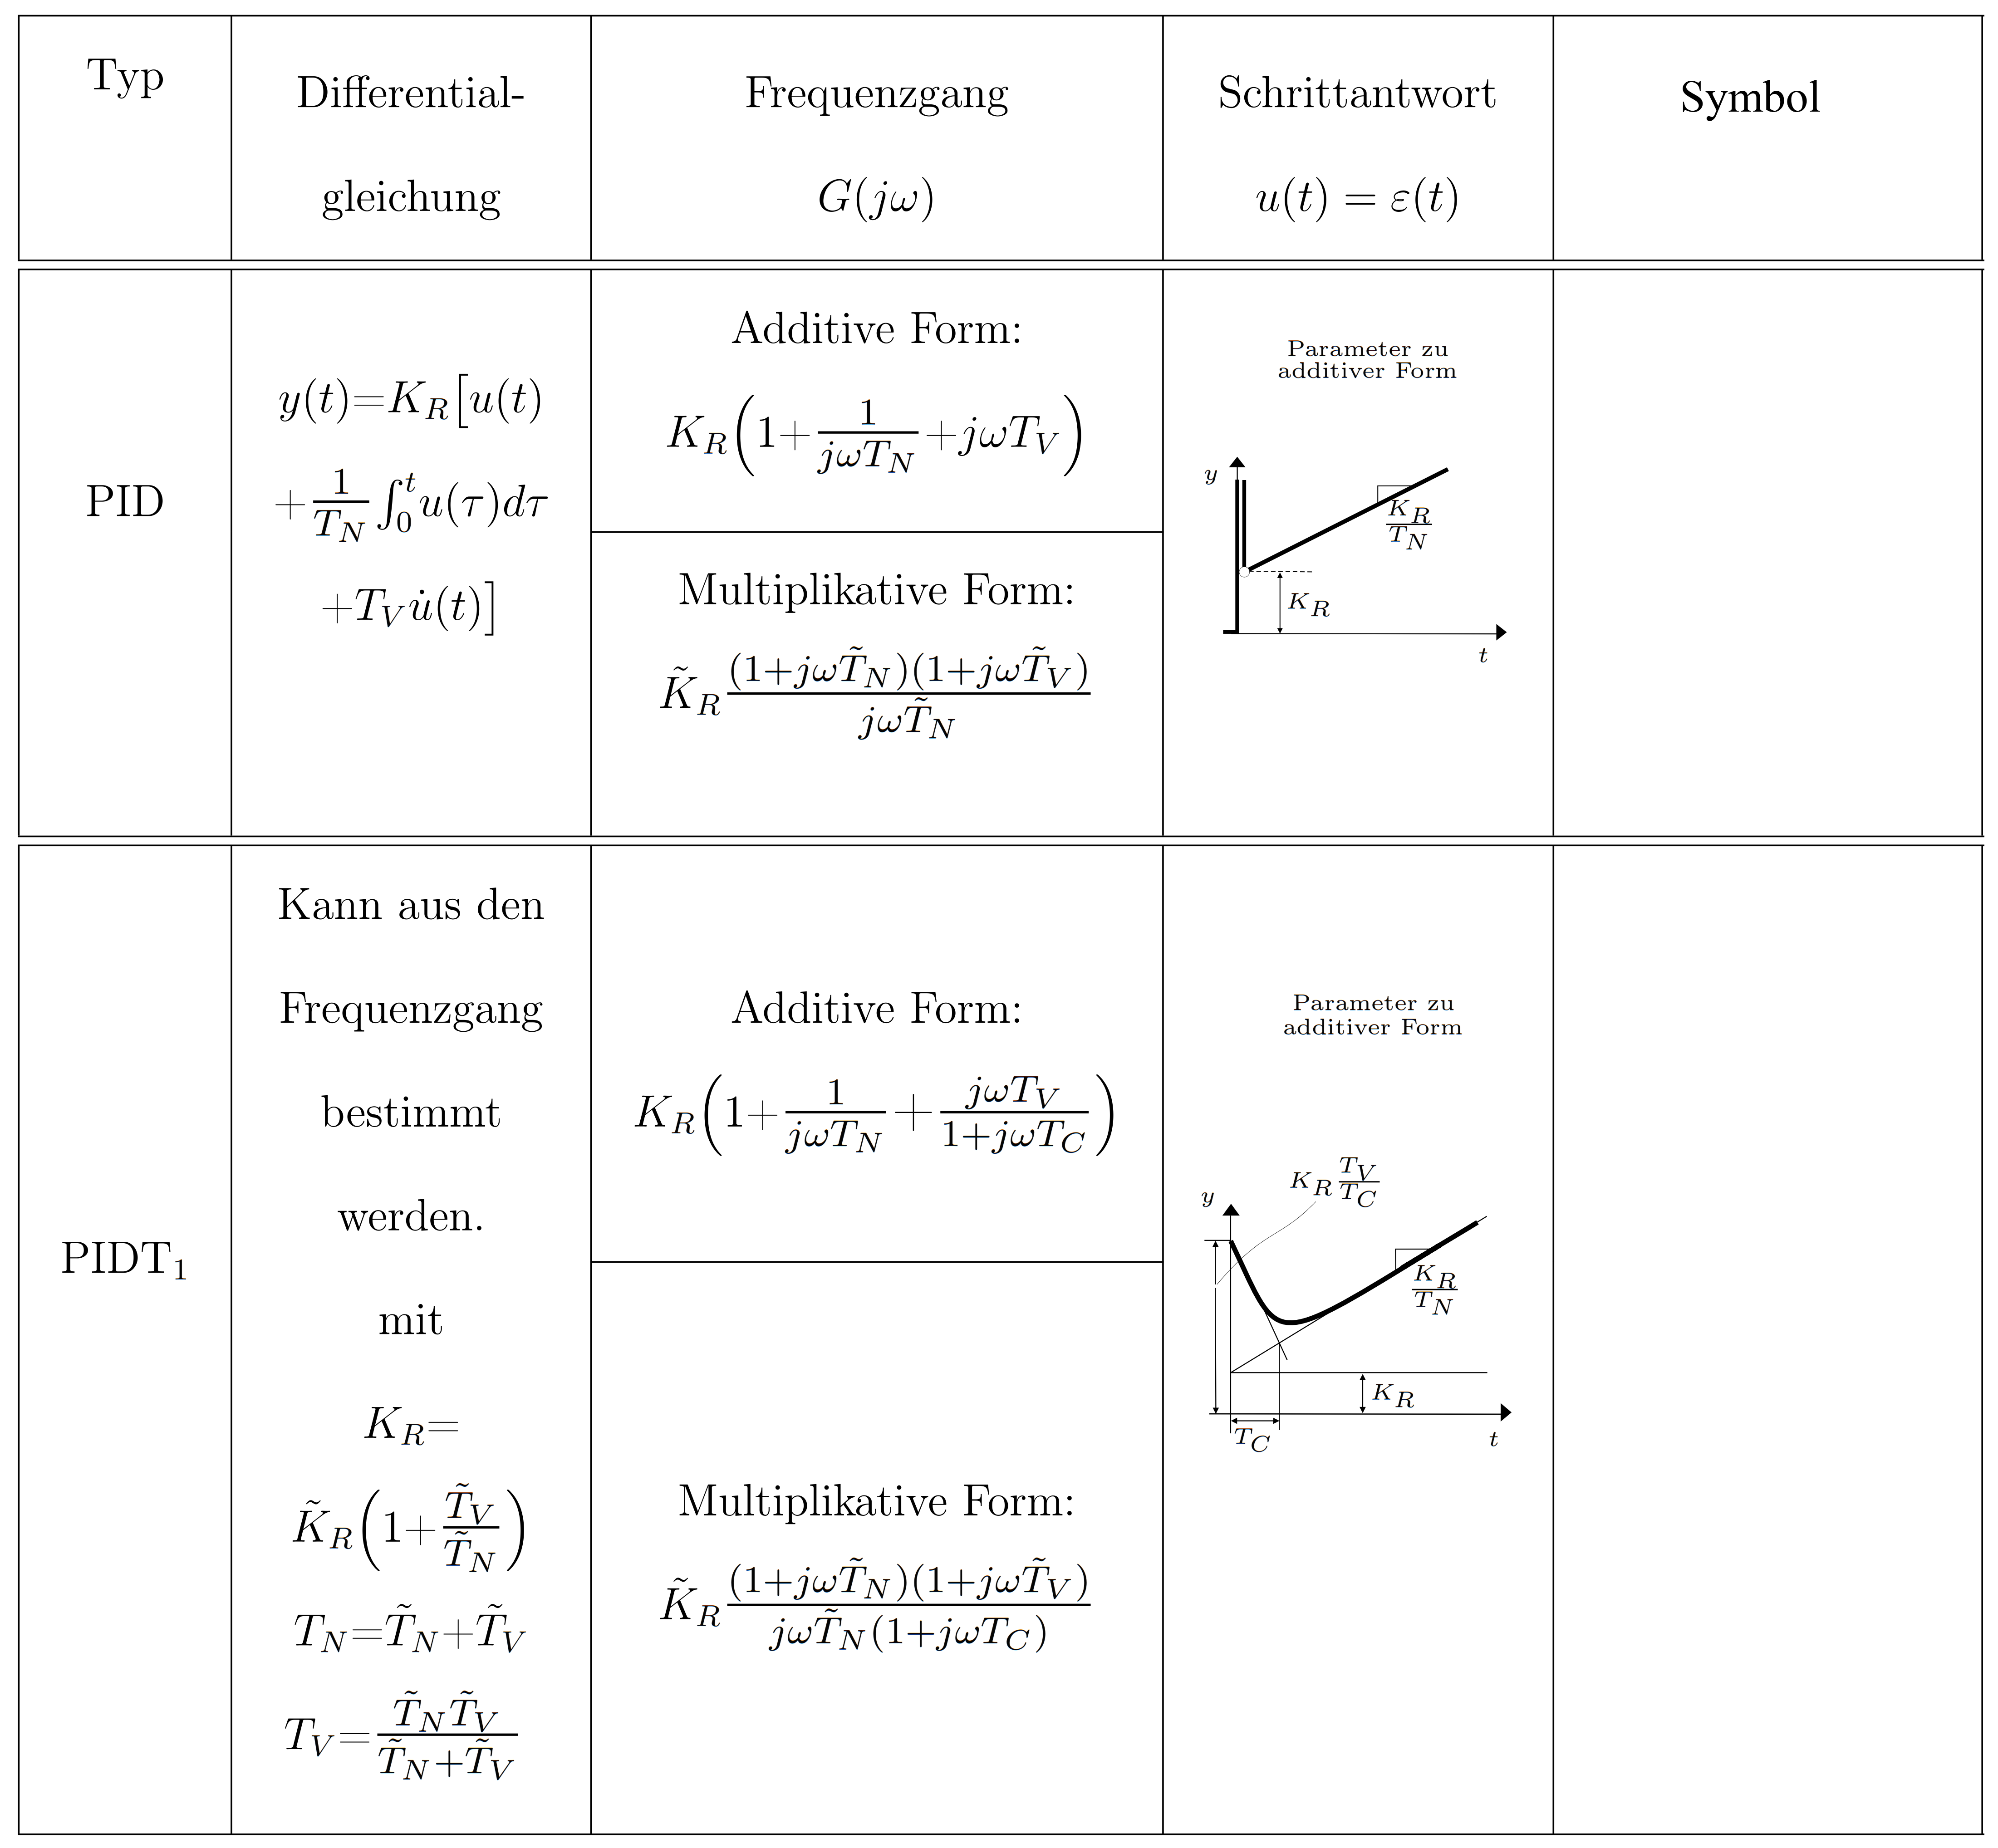
\includegraphics[width=12 cm]{./bilder/glieder5.png} \newpage

%\vspace{0.5cm}
%\rotatebox{90}{
%  \begin{minipage}[]{23cm}
%	\begin{tabular}{|l|l|l|l|l|l|}
%    	\hline
%    	\textbf{Benennung}	&\textbf{Funktion}	&\textbf{UTF}	& \textbf{Sprungantw.}	
%    	&\textbf{Verlauf Sprungantw.}	&\textbf{Symbol}\\
%    	\hline
%    	\hline
%    	\textbf{P-Glied} \formelbuch{26} & $y(t)=K u(t)$	& K & K
%    	&\begin{minipage}{2.4cm}
%         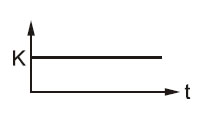
\includegraphics[width=2.4cm,trim=0 0 -5 -5]{./bilder/verlaufP.jpg}
%         \end{minipage}
%    	&\begin{minipage}{2.4cm}
%         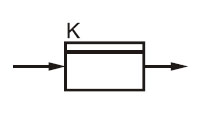
\includegraphics[width=2.4cm]{./bilder/p-Glied.jpg}
%         \end{minipage}\\
%    	\hline
%    	%
%    	\textbf{I-Glied} \formelbuch{29} &
%    	\parbox{3cm}{$\dot{y}= K u(t)$\\
%    				$y=K\int \limits_0^t u(t) dt$\\}
%    				&$\dfrac{K}{s}$ & Kt
%    	&\begin{minipage}{2.4cm}
%         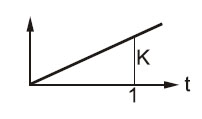
\includegraphics[width=2.4cm,trim=0 0 -5 -5]{./bilder/verlaufI.jpg}
%         \end{minipage}
%    	&\begin{minipage}{2.4cm}
%         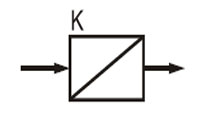
\includegraphics[width=2.4cm]{./bilder/I-Glied.jpg}
%         \end{minipage}\\
%    	\hline	
%    	\textbf{Totzeit-Glied} \formelbuch{30}	
%    	&$y(t)=u(t-T_t)$	&$e^{-T_t s}$	&$K \cdot u(t-T_t)$
%    	&\begin{minipage}{2.4cm}
%         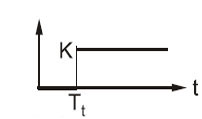
\includegraphics[width=2.4cm,trim=0 0 -5 -5]{./bilder/verlaufTt.jpg}\\
%         \end{minipage}
%    	&\begin{minipage}{2.4cm}
%         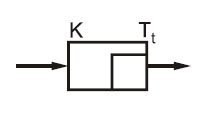
\includegraphics[width=2.4cm]{./bilder/Tt-Glied.jpg}
%         \end{minipage}\\
%		\hline
%    	 \begin{minipage}{4cm}
%			\vspace{0.2cm}
%			\textbf{PT$_1$-Glied} \formelbuch{31}\\
%			%    	   	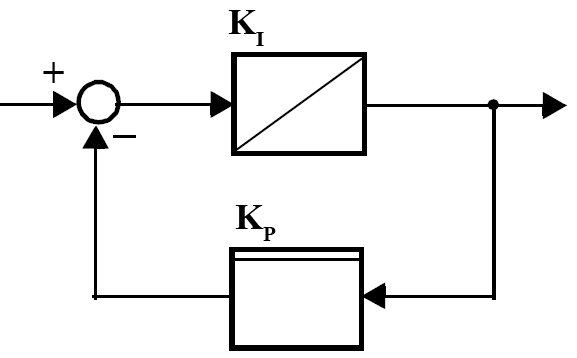
\includegraphics[width=4cm]{./bilder/PT1.png}   
%         \end{minipage}
%		 &\parbox{3cm}{$T\dot{y}+y=K u(t)$\\\\
%		 $T = \dfrac{1}{K_i \cdot K_p}$\\
%		 $K = \dfrac{1}{K_p}$}	 
%		 &$\dfrac{K}{1+Ts}$
%    	 &$K(1-e^{-\frac{t}{T}})$
%    	 &\begin{minipage}{2.4cm}
%         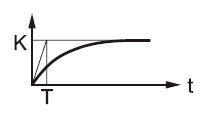
\includegraphics[width=2.3cm]{./bilder/verlaufPT1.jpg}
%         \end{minipage}
%    	&\begin{minipage}{2.4cm}
%         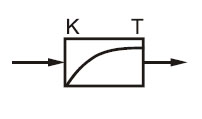
\includegraphics[width=2.3cm]{./bilder/Pt1-Glied.jpg}
%         \end{minipage}\\
%    	\hline
%    	\multicolumn{6}{|l|}{
%    		\parbox{18cm}{\textbf{PT$_1$-Glied mit Grundelementen} ($K$: Verstärkung; $T$: Zeitkonstante):\\
%    				\begin{minipage}{10cm}
%    				    \hspace*{4cm}
%    				    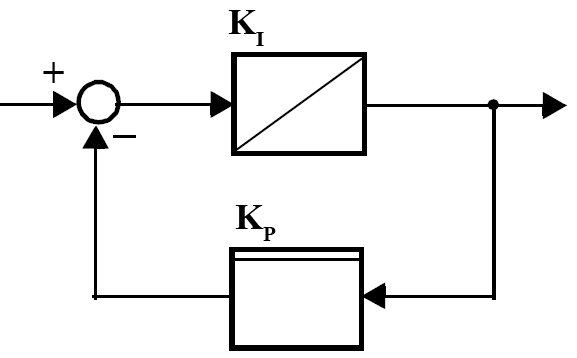
\includegraphics[width=4cm]{./bilder/PT1.png}
%    				\end{minipage}
%    				\begin{minipage}{7cm}
%    					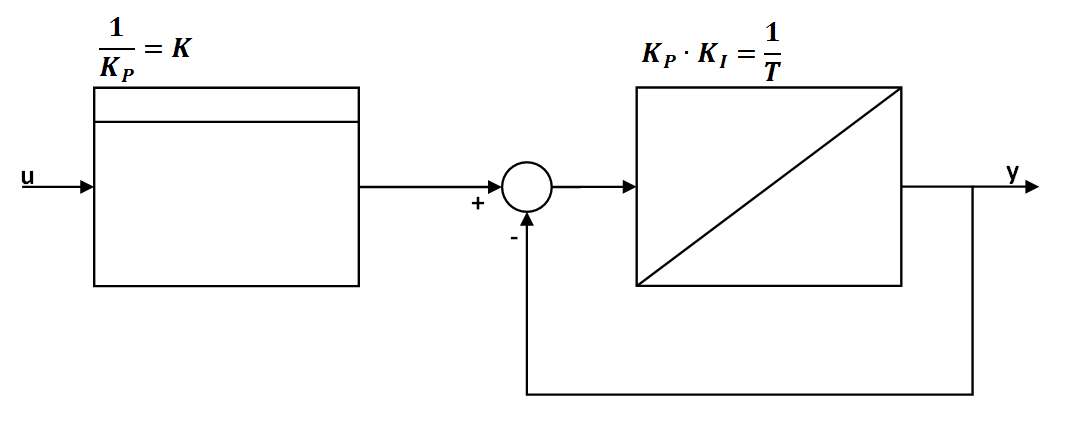
\includegraphics[width=6cm]{./bilder/PT1_2.png}
%    				\end{minipage}
%    		}
%    	}\\
%    	\hline
%		\textbf{PT$_2$-Glied} \formelbuch{34}	
%    	&$T^2\cdot\ddot{y}(t)+2\zeta T\cdot \dot{y}(t)+y(t)=K\cdot u(t)$	
%    	&$\dfrac{K}{1+2dTs+T^2s^2}$	
%    	& siehe unten *
%    	&	\begin{minipage}{1.5 cm}
%         	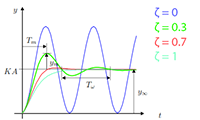
\includegraphics[width=2.2cm,trim=0 0 -3 -5]{./bilder/pt2.png}
%         	\end{minipage}
%         	\begin{minipage}{0.9 cm}
%         	Test
%         	\end{minipage}
%        \hline 
%    	&\begin{minipage}{2.4cm}
%         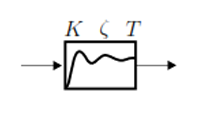
\includegraphics[width=2.4cm]{./bilder/pt2_symbol.png}
%         \end{minipage}\\
%		\hline
%		\textbf{D-Glied} \formelbuch{37}	
%    	&$y(t)= K\cdot \dot{u}(t)$	
%    	&$K \cdot s$	
%    	&$KA \cdot \delta(t)$
%    	&\begin{minipage}{2.4cm}
%         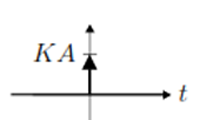
\includegraphics[width=2.2cm,trim=0 0 -3 -5]{./bilder/d-glied.png}\\
%         \end{minipage}
%    	&\begin{minipage}{2.4cm}
%         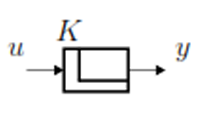
\includegraphics[width=2.4cm]{./bilder/d-glied_symbol.png}
%         \end{minipage}\\
%		\hline
%	\textbf{DT$_1$-Glied} \formelbuch{38}	
%    	&$T\cdot \dot{y}(t)+y(t)= K\cdot \dot{u}(t)$	
%    	&$\frac {K \cdot s} {1+Ts}$	
%    	&$\frac {K\cdot A} {T \cdot e^-\frac {t}{T}}$
%    	&\begin{minipage}{2.4cm}
%         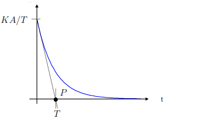
\includegraphics[width=2.2cm,trim=0 0 -3 -5]{./bilder/dt1-glied.png}\\
%         \end{minipage}
%    	&\begin{minipage}{2.4cm}
%         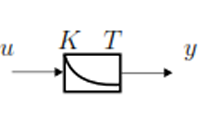
\includegraphics[width=2.4cm]{./bilder/dt1-glied_symbol.png}
%         \end{minipage}\\
%		\hline
%    \end{tabular}
%    \\\\\\   
%         \begin{minipage}[t]{16 cm}
%         * $\left\{\begin{array}{ll}K-\frac{K}{T_1-T_2}\left[T_1e^{-\frac{t}{T_1}}-T_2e^{-\frac{t}{T_2}}\right] & \zeta > 1 (aperiodischer Fall)\\ K-\frac{K}{\sqrt{1-\zeta^2}}e^{-\frac{\zeta}{T}t}\cdot \sin \left[\frac{\sqrt{1-\zeta^2}}{T}t+\arctan \frac{\sqrt{1-\zeta^2}}{\zeta}\right] & \zeta < 1 (periodischer Fall) \\ K-K\left[1+\frac{t}{T}\right]e^{-\frac{t}{T}} & \zeta = 1 (aperiodischer Grenzfall) \end{array}\right.$ 
%         \end{minipage} 
%         \begin{minipage}[t]{8 cm}
%         mit $T_1,2 = \frac{T}{d\pm \sqrt{d^2-1}}$
%         \end{minipage} 
%   \end{minipage}     
%    } 
    
    \begin{multicols}{3}
    \textbf{P-Glied (nicht inv. Op-Amp)} \\
    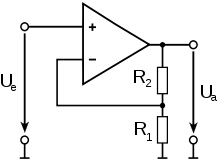
\includegraphics[height=2.5cm]{./bilder/OP-Amp.png} \\
    $K = 1 + \frac{R_2}{R_1}$ 
    \columnbreak
	\textbf{P-Glied (inv. Op-Amp)} \\ 
	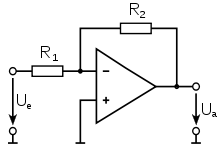
\includegraphics[height=2.5cm]{./bilder/OP-InvAmp.png} \\
	$K=-\frac{R_2}{R_1}$
    \columnbreak     
    \textbf{I-Glied} \\ 
    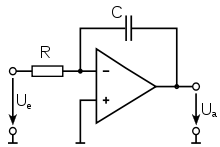
\includegraphics[height=2.5cm]{./bilder/OP-Integrator.png}\\
    $K = - \frac{1}{R \cdot C}$
    \end{multicols}  
    \begin{minipage}{16cm}
    \subsection{Stationäre Signale}
	Für den stationären Fall gelten folgende Bedingungen:
	\begin{itemize}
    	\item \textbf{Integratoren} haben am \textbf{Eingang Null}.
    	\item \textbf{Integratoren} haben am \textbf{Ausgang} einen \textbf{beliebigen Wert}.
    	\item \textbf{Totzeitglieder} werden kurzgeschlossen.
    	\item \textbf{PT$_1$-Glieder} wirken als \textbf{P-Glieder} mit $K_P = K_{PT_1}$ behandelt.
    	\item (\textbf{Fehlersignale} werden jeweils als \textbf{Null} angenommen.) \textbf{Mit Vorsicht annehmen}
  	\end{itemize}
  	\end{minipage} \\
	\subsection{Zwei- und Dreipunktregler}
	\subsection{Stetigähnliche Regler}
		\subsubsection{Rückkopplung des Reglers}
		\begin{minipage}{9cm}
		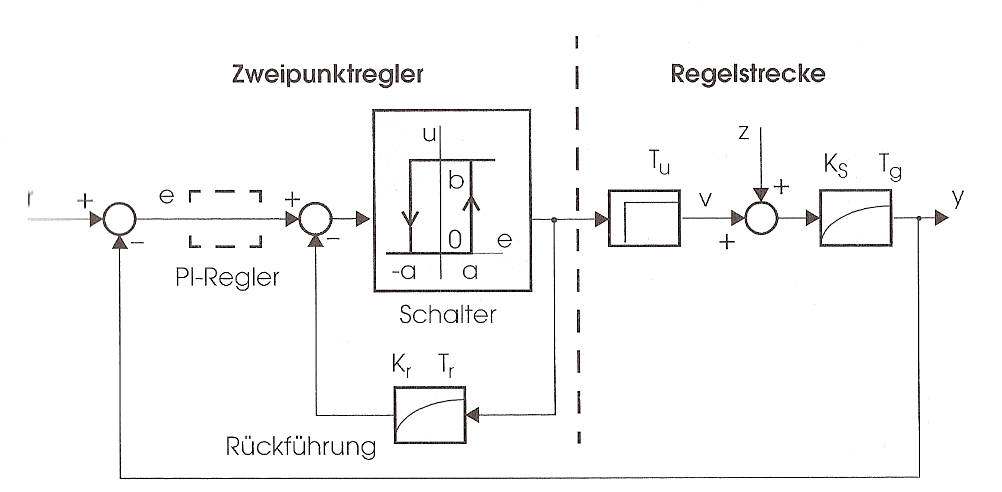
\includegraphics[width=8.5cm]{./bilder/ZweipunktreglerMitRueckfuehrung.jpg}
        \end{minipage}
		\begin{minipage}{7.5cm}
        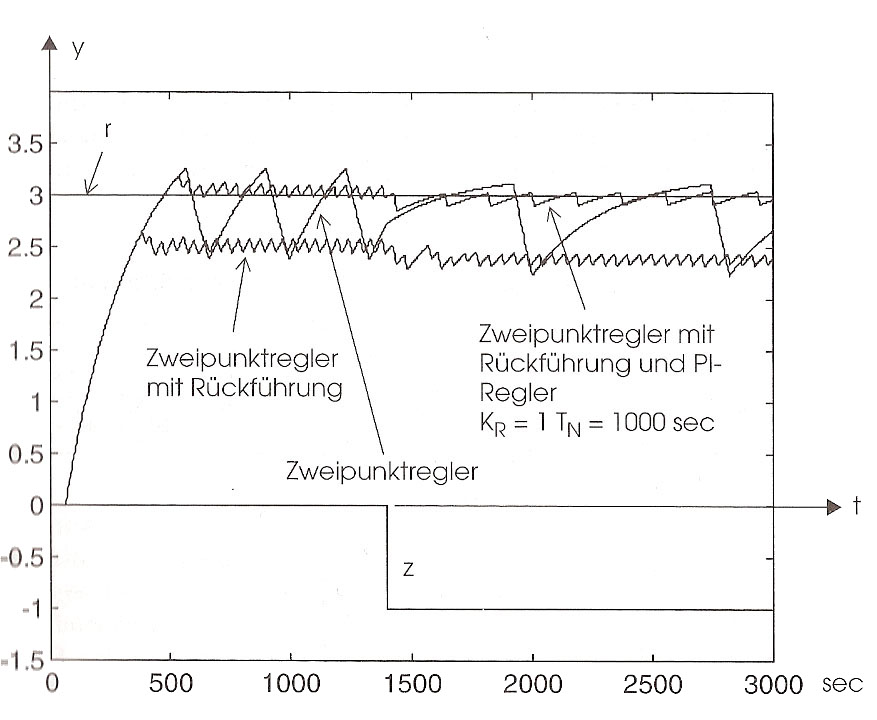
\includegraphics[width=7cm]{./bilder/ZweipunktreglerMitRueckfuehrung_dia.jpg}
        \end{minipage}\\
		Die Rückkopplung mit einem $PT_1$-Glied über dem Zweipunkteregler bewirkt
		einen bedeutend kleineren Rippel. Leider ist der Mittelwert noch unterhalb des
		Sollwertes. Mithilfe eines PI-Reglers vor dem Zweipunkteregler, kann der IST-Wert
		angehoben werden.
	\subsubsection{Dreipunktregler}
		\begin{minipage}{9cm}
		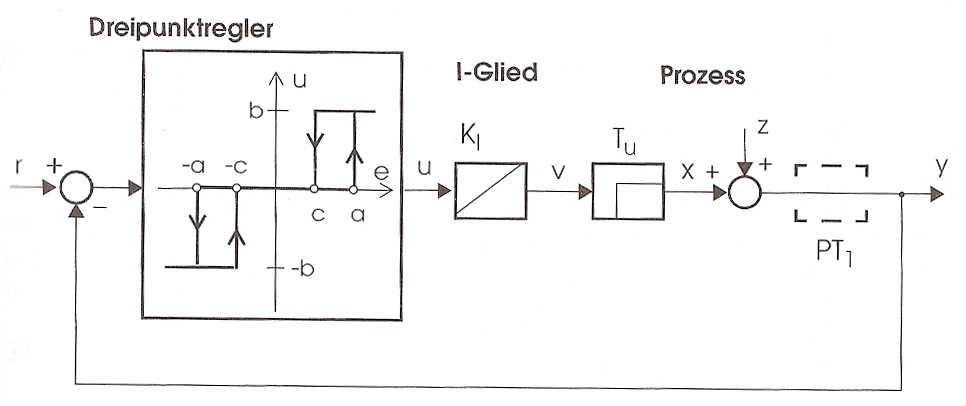
\includegraphics[width=9cm]{./bilder/Dreipunktregler.jpg}
        \end{minipage}
		\begin{minipage}{7.5cm}
        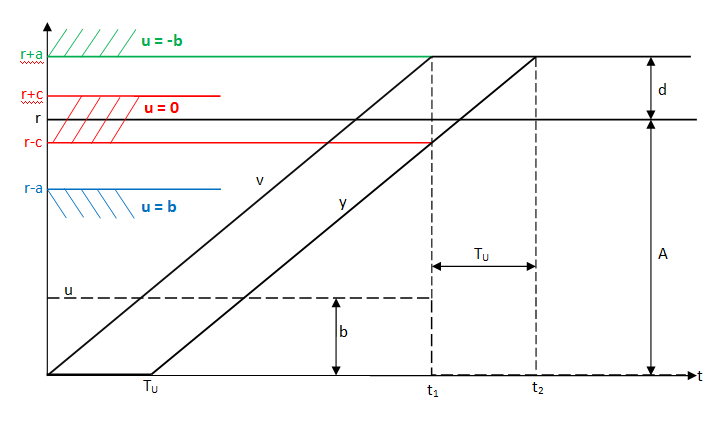
\includegraphics[width=7.5cm]{./bilder/Dreipunktregler_dia.png}
        \end{minipage}\\
		gewünscht: $d = 0 \rightarrow c = K_I \cdot T_u \cdot b$\\
		Falls mit PT$_1$-Glied $\rightarrow c = K_I \cdot K_s \cdot b (T_u + T_G)$
	\subsubsection{Zweipunktregler}
		\begin{minipage}{3cm}
 		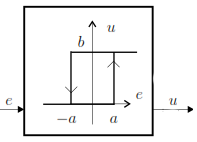
\includegraphics[height=3cm]{./bilder/Zweipunkteregler.png}
        \end{minipage}
		\begin{minipage}{15cm}
        Ein Zweipunktregler ist ein unstetig arbeitender Regler mit zwei
        Ausgangszuständen. Je nachdem, ob der Istwert über oder unter dem
        Sollwert liegt, wird der erste oder der zweite Ausgangszustand
        eingenommen. 
        \end{minipage}
	\textbf{Beispiele von Zweipunkte-Reglerschaltungen:}\\ \\
		\textbf{Zweipunktregler mit symmetrischer Kennlinie \formelbuch{52}} \\
		\begin{minipage}{9cm}
			\vspace{.5cm}        
	 		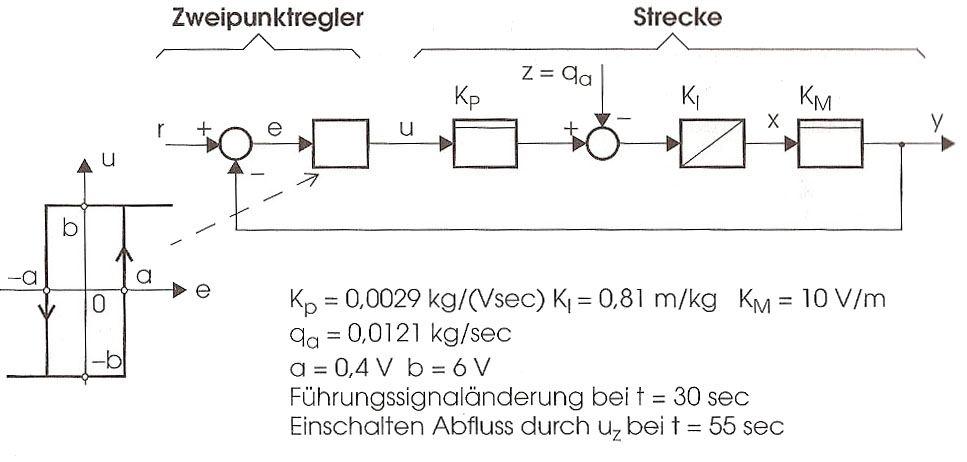
\includegraphics[width=9cm]{./bilder/Zweipunktregler-b+b2.jpg}\\
			Die Anstiegszeit beträgt nach dem Einschwingvorgang:\\
			$t_{ein}=\frac{2a}{(b K_p - q_a)K_i K_m}$ \\ \\
			Die Abfallszeit beträgt nach dem Einschwingvorgang:\\
			$t_{aus}=\frac{2a}{(b K_p + q_a)K_i K_m}$
        \end{minipage}
		\begin{minipage}{9cm}
			\vspace{.5cm}        
			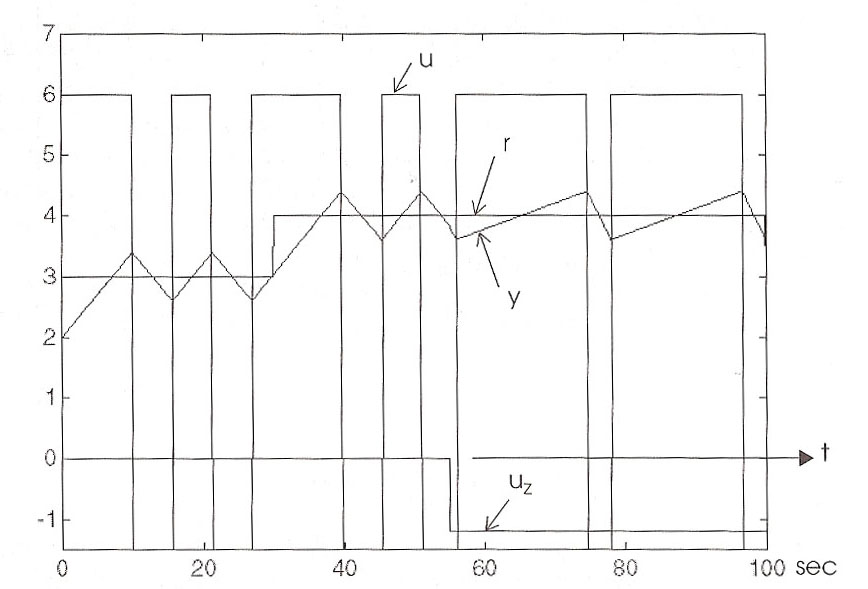
\includegraphics[width=9cm]{./bilder/Zweipunktregler-b+b_dia.jpg}
        \end{minipage}\\
         Einfüllen mit Abfluss: $y = y_0 + K_M \cdot K_I(K_p \cdot b - Q_a)(t-t_0); \qquad$ 
         Entleeren: $y=y_1 + K_M \cdot K_I(K_p(-b) - Q_a)(t-t_0)$
    
	\vspace{.5cm}
		\textbf{Zweipunktregler an ausgleichender Strecke \formelbuch{53}} \\
		\begin{minipage}{9cm}
 		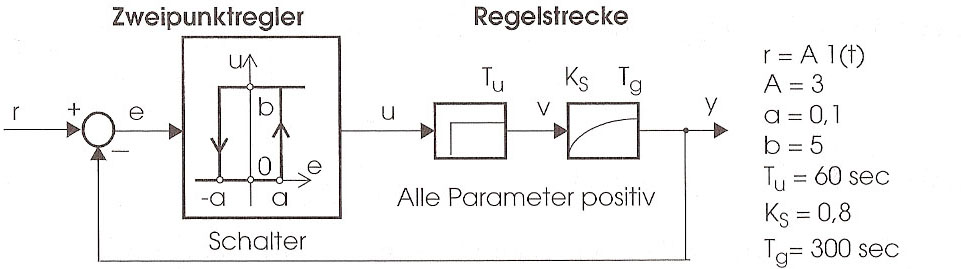
\includegraphics[width=9cm]{./bilder/ZweipunktreglerTotglied2.jpg}\\
			Die Anstiegszeit beträgt nach dem Einschwingvorgang:
			$t_{ein}$=$T_g\ln(\frac{e^{-\frac{T_u}{T_g}}(A-a)-b K_s}{A+a-b K_s})+T_u$\\ \\
			Die Abfallszeit beträgt nach dem Einschwingvorgang:
			$t_{aus}$=$T_g\ln(\frac{A+a-b
			K_s+\frac{b K_s}{e^{-\frac{T_u}{T_g}}}}{A-a})$\\
        \end{minipage}
		\begin{minipage}{9cm}
		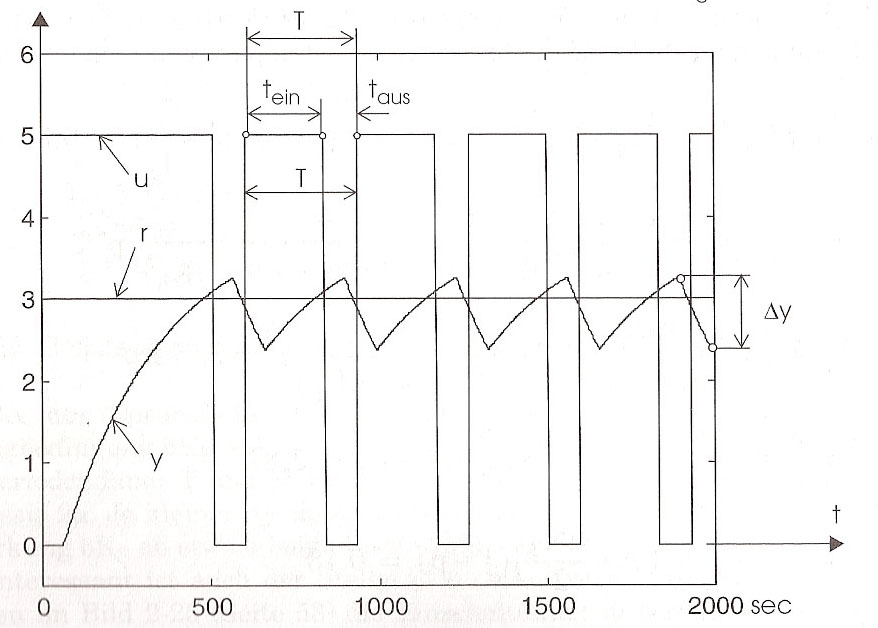
\includegraphics[width=9cm]{./bilder/ZweipunktreglerTotglied_dia.jpg}			
        \end{minipage}
    
 	$\Delta y = b\cdot K_s - e^{-\frac{T_u}{T_G}}(b\cdot K_s - 2a); \qquad$
	$y_m = \frac{y_{min}+y_{max}}{2}=e^{-\frac{T_u}{T_G}}\cdot A + \frac{b\cdot K_s}{2}(1-e^{-\frac{T_u}{T_G}}$

